\documentclass[11pt,paper=a4,answers]{exam}
\usepackage{graphicx,lastpage}
\usepackage{upgreek}
\usepackage{censor}
\usepackage{gensymb}
\usepackage{amsmath}
\usepackage{multicol}
\usepackage{enumitem}
 \usepackage{pgfplots}
\pgfplotsset{compat=1.18}
\usepackage{tasks}
\usepackage{adjustbox}
\usepackage{xcolor}
\usepackage{tfrupee}
\setlength{\voffset}{0.25in}
\usepackage{tabularx}
\newcolumntype{Y}{>{\centering\arraybackslash}X}
%==============================================================
% Customise Non-Essential Packages Below
% =============================================================
\usepackage[most]{tcolorbox}
\usepackage{eso-pic}
\usepackage{tikz}
\AddToShipoutPictureBG{%
\begin{tikzpicture}[remember picture,overlay]
\foreach \x in {-8,-4,0,4,8,12,16,20}
\foreach \y in {-8,-4,0,4,8,12,16,20} {
\node[opacity=0.05,rotate=45,anchor=center] at ([xshift=\x cm,yshift=\y cm]current page.center) {%
\begin{minipage}{2cm}
\centering
\includegraphics[width=2cm]{images/logo_black.png}\\
\small preppeo.com
\end{minipage}%
};
}
\end{tikzpicture}%
}
\printanswers

%==============================================================
% Customise Non-Essential Packages Above
% =============================================================
\definecolor{svgray}{rgb}{0.90, 0.90, 0.90}
\graphicspath{{images/}}

\usepackage[normalem]{ulem}
\renewcommand\ULthickness{1pt}   %%---> For changing thickness of underline
\setlength\ULdepth{3.5ex}%\maxdimen ---> For changing depth of underline
\renewcommand{\baselinestretch}{1}
\chead{
\includegraphics[scale=0.1,height=2cm ]{logo.png}
}
\pagestyle{empty}

\pagestyle{headandfoot}
\headrule
\cfoot{W: https://preppeo.com; M: +91-8130711689}

\begin{document}
%==============================================================
% Customise Question paper details below this
% =============================================================
\begin{center}
    \centering
    \renewcommand{\arraystretch}{1.5}
    \begin{tabularx}{\textwidth}{YYY}
    & \normalsize\bf{{\Large{{Quantitative Reasoning}}}} & \\
    By Preppeo & \normalsize\bf{MOCK } & GRE\\
    \normalsize{\textbf{Questions:} 15 ( Section 2 : 15} & \normalsize{\textbf{Marks:} 15 } & \normalsize{\textbf{Time:}  minutes } \\
    \end{tabularx}
\end{center}
\par\noindent\rule{\textwidth}{1pt}
% =============================================================
% Customise Question paper details above this
% =============================================================

\begin{questions}
\pointsinrightmargin
\pointsdroppedatright
\marksnotpoints
\pointpoints{mark}{marks}
\pointformat{\boldmath\themarginpoints}
\bracketedpoints

% =============================================================
% Question Begin
% =============================================================

\section*{Section 2 - Mock 8 Set 2 (Very Very Hard)}

% --- QUANTITY COMPARISON (5 QUESTIONS) ---

%Q: 1
\question
Let $S$ be a set of $n$ distinct integers. The range of $S$ is $r$. A new set $T$ is created by multiplying every element in $S$ by $-3$ and then adding 5.
\vspace{5pt}
\textbf{Quantity A: } The range of set $T$ \\
\vspace{5pt}
\textbf{Quantity B: } $3r$

\begin{tasks}(1)
\task[A)] Quantity A is greater
\task[B)] Quantity B is greater
\task[C)] The two quantities are equal
\task[D)] The relationship cannot be determined
\end{tasks}

\begin{solution}
Let the maximum value in set $S$ be $S_{max}$ and the minimum be $S_{min}$. The range is $r = S_{max} - S_{min}$.
\vspace{5pt}
\begin{center}
When elements are multiplied by a negative number $(-3)$, the order is reversed.
\vspace{5pt}
The new maximum $T_{max} = (-3 \times S_{min}) + 5$.
\vspace{5pt}
The new minimum $T_{min} = (-3 \times S_{max}) + 5$.
\vspace{10pt}
$\text{Range of } T = T_{max} - T_{min}$
\vspace{5pt}
$\text{Range of } T = [(-3 \times S_{min}) + 5] - [(-3 \times S_{max}) + 5]$
\vspace{5pt}
$\text{Range of } T = -3S_{min} + 5 + 3S_{max} - 5$
\vspace{5pt}
$\text{Range of } T = 3(S_{max} - S_{min}) = 3r$
\end{center}
\vspace{5pt}
Quantity A is $3r$ and Quantity B is $3r$. They are equal.

Answer: \colorbox{yellow!100}{C}
\end{solution}

\vspace{1cm}

%Q: 2
\question
$k$ is a positive integer.
\vspace{5pt}
\textbf{Quantity A: } The remainder when $7^{4k+2}$ is divided by 10 \\
\vspace{5pt}
\textbf{Quantity B: } The remainder when $3^{4k+2}$ is divided by 10

\begin{tasks}(1)
\task[A)] Quantity A is greater
\task[B)] Quantity B is greater
\task[C)] The two quantities are equal
\task[D)] The relationship cannot be determined
\end{tasks}

\begin{solution}
The remainder when divided by 10 is the units digit. 
\vspace{5pt}
\begin{center}
Cycle for 7: $7, 9, 3, 1$. (Length 4).
\vspace{5pt}
The exponent $4k+2$ has a remainder of 2 when divided by 4.
\vspace{5pt}
The units digit is the 2nd in the cycle: 9.
\vspace{10pt}
Cycle for 3: $3, 9, 7, 1$. (Length 4).
\vspace{5pt}
The exponent $4k+2$ has a remainder of 2 when divided by 4.
\vspace{5pt}
The units digit is the 2nd in the cycle: 9.
\end{center}
\vspace{5pt}
Both remainders are 9.

Answer: \colorbox{yellow!100}{C}
\end{solution}

\vspace{1cm}

%Q: 3
\question
A container holds 12 red marbles and 18 blue marbles. Two marbles are drawn at random without replacement.
\vspace{5pt}
\textbf{Quantity A: } The probability that both marbles are blue \\
\vspace{5pt}
\textbf{Quantity B: } $1/3$

\begin{tasks}(1)
\task[A)] Quantity A is greater
\task[B)] Quantity B is greater
\task[C)] The two quantities are equal
\task[D)] The relationship cannot be determined
\end{tasks}

\begin{solution}
\begin{center}
Total marbles $= 12 + 18 = 30$
\vspace{5pt}
$P(\text{1st is blue}) = 18/30 = 3/5$
\vspace{5pt}
$P(\text{2nd is blue}) = 17/29$ (No replacement)
\vspace{10pt}
$P(\text{Both blue}) = \dfrac{3}{5} \times \dfrac{17}{29} = \dfrac{51}{145}$
\vspace{5pt}
Convert to decimal: $51 \div 145 \approx 0.3517$
\vspace{5pt}
Quantity B: $1/3 \approx 0.3333$
\end{center}
\vspace{5pt}
Quantity A is greater.

Answer: \colorbox{yellow!100}{A}
\end{solution}

\vspace{1cm}

%Q: 4
\question
$a$ and $b$ are integers such that $a^2 - b^2 = 21$ and $a > b > 0$.
\vspace{5pt}
\textbf{Quantity A: } $a \times b$ \\
\vspace{5pt}
\textbf{Quantity B: } 12

\begin{tasks}(1)
\task[A)] Quantity A is greater
\task[B)] Quantity B is greater
\task[C)] The two quantities are equal
\task[D)] The relationship cannot be determined
\end{tasks}

\begin{solution}
Factor the difference of squares: $(a-b)(a+b) = 21$.
\vspace{5pt}
\begin{center}
Case 1: $a-b=1$ and $a+b=21 \implies 2a=22 \implies a=11, b=10$.
\vspace{5pt}
$a \times b = 110$.
\vspace{10pt}
Case 2: $a-b=3$ and $a+b=7 \implies 2a=10 \implies a=5, b=2$.
\vspace{5pt}
$a \times b = 10$.
\end{center}
\vspace{5pt}
Since $110 > 12$ but $10 < 12$, the relationship cannot be determined.

Answer: \colorbox{yellow!100}{D}
\end{solution}

\vspace{1cm}

%Q: 5
\question
\begin{center}
\begin{tikzpicture}
    \draw[thick] (0,0) -- (4,0) node[midway, below] {$s$} -- (4,4) -- (0,4) -- cycle;
    \draw[thick, dashed] (0,4) -- (4,0);
    \draw[thick, blue] (2,4) -- (4,2);
    \node at (1.2, 1.2) {$T_1$};
    \node at (3.4, 3.4) {$T_2$};
\end{tikzpicture}
\end{center}
$T_1$ is formed by a diagonal of square $s$. $T_2$ is formed by connecting the midpoints of adjacent sides.
\vspace{5pt}
\textbf{Quantity A: } Area of $T_1$ \\
\vspace{5pt}
\textbf{Quantity B: } $4 \times \text{Area of } T_2$

\begin{tasks}(1)
\task[A)] Quantity A is greater
\task[B)] Quantity B is greater
\task[C)] The two quantities are equal
\task[D)] The relationship cannot be determined
\end{tasks}

\begin{solution}
\begin{center}
$\text{Area } T_1 = \dfrac{1}{2} s^2$
\vspace{5pt}
$T_2$ legs are $s/2$. $\text{Area } T_2 = \dfrac{1}{2} \times \dfrac{s}{2} \times \dfrac{s}{2} = \dfrac{s^2}{8}$
\vspace{10pt}
$4 \times \text{Area } T_2 = 4 \times \dfrac{s^2}{8} = \dfrac{s^2}{2}$
\end{center}
\vspace{5pt}
Both are equal.

Answer: \colorbox{yellow!100}{C}
\end{solution}

\vspace{1cm}

% --- MCQ SINGLE CHOICE (5 QUESTIONS) ---

%Q: 6
\question
If $3^{x+1} - 3^x = 486$, what is the value of $x$?

\begin{tasks}(1)
\task[A)] 4 \task[B)] 5 \task[C)] 6 \task[D)] 7 \task[E)] 8
\end{tasks}

\begin{solution}
\begin{center}
Factor out $3^x$: $3^x(3 - 1) = 486$
\vspace{5pt}
$3^x(2) = 486 \implies 3^x = 243$
\vspace{5pt}
$243 = 3^5 \implies x = 5$
\end{center}

Answer: \colorbox{yellow!100}{B}
\end{solution}

\vspace{1cm}

%Q: 7
\question
A contractor surrounds a circular pool of radius $r$ with a 2-meter stone walkway. If the walkway area is $44\pi$, what is $r$?

\begin{tasks}(1)
\task[A)] 8 \task[B)] 10 \task[C)] 12 \task[D)] 14 \task[E)] 16
\end{tasks}

\begin{solution}
\begin{center}
Outer radius $= r + 2$.
\vspace{5pt}
$\pi(r+2)^2 - \pi r^2 = 44\pi$
\vspace{5pt}
$r^2 + 4r + 4 - r^2 = 44 \implies 4r = 40 \implies r = 10$
\end{center}

Answer: \colorbox{yellow!100}{B}
\end{solution}

\vspace{1cm}

%Q: 8
\question
Which of the following is equivalent to $\dfrac{-2}{\sqrt{n} - 1 - \sqrt{n} + 1}$? 

\begin{tasks}(1)
\task[A)] $-1$ \task[B)] $1$ \task[C)] $2(\sqrt{n-1} + \sqrt{n+1})$ \task[D)] $\sqrt{n-1} + \sqrt{n+1}$ \task[E)] $1/n$
\end{tasks}

\begin{solution}
To simplify the expression from the provided logic:
\vspace{5pt}
\begin{center}
$\dfrac{-2}{\sqrt{n-1} - \sqrt{n+1}}$
\vspace{5pt}
Multiply numerator and denominator by the conjugate $(\sqrt{n-1} + \sqrt{n+1})$:
\vspace{10pt}
$\dfrac{-2(\sqrt{n-1} + \sqrt{n+1})}{(\sqrt{n-1} - \sqrt{n+1})(\sqrt{n-1} + \sqrt{n+1})}$
\vspace{5pt}
Denominator becomes: $(n-1) - (n+1) = n - 1 - n - 1 = -2$
\vspace{10pt}
The expression simplifies to: $\dfrac{-2(\sqrt{n-1} + \sqrt{n+1})}{-2} = \sqrt{n-1} + \sqrt{n+1}$
\end{center}

Answer: \colorbox{yellow!100}{D}
\end{solution}

\vspace{1cm}

%Q: 9
\question
How many ways to arrange 6 people in a row if 2 refuse to sit together?

\begin{tasks}(1)
\task[A)] 120 \task[B)] 240 \task[C)] 480 \task[D)] 720 \task[E)] 840
\end{tasks}

\begin{solution}
\begin{center}
Total arrangements $= 6! = 720$.
\vspace{5pt}
Arrangements where they are together $= (5! \times 2) = 240$.
\vspace{5pt}
Apart $= 720 - 240 = 480$.
\end{center}

Answer: \colorbox{yellow!100}{C}
\end{solution}

\vspace{1cm}

%Q: 10
\question
In a collegiate department, 60\% play a winter sport and 40\% of those also play spring. If 120 play both, what is the total number of athletes?

\begin{tasks}(1)
\task[A)] 300 \task[B)] 400 \task[C)] 500 \task[D)] 600 \task[E)] 800
\end{tasks}

\begin{solution}
\begin{center}
Let $T$ be total. Winter athletes $= 0.60T$.
\vspace{5pt}
Both $= 0.40 \times (0.60T) = 0.24T$.
\vspace{5pt}
$0.24T = 120 \implies T = 120 / 0.24 = 500$.
\end{center}

Answer: \colorbox{yellow!100}{C}
\end{solution}

\vspace{1cm}

% --- MCQ MULTIPLE CHOICE (1 QUESTION) ---

%Q: 11
\question
If $k$ is a positive integer, which could be the remainder of $7^k$ divided by 100?
Indicate \textbf{all} such values.

\begin{tasks}(1)
\task[A)] 07 \task[B)] 49 \task[C)] 43 \task[D)] 01
\end{tasks}

\begin{solution}
\begin{center}
$7^1=07, 7^2=49, 7^3=343 \to 43, 7^4=2401 \to 01$.
\end{center}
The cycle of the last two digits consists of these four values.

Answer: \colorbox{yellow!100}{A, B, C, D}
\end{solution}

\vspace{1cm}

% --- INPUT QUESTION (1 QUESTION) ---

%Q: 12
\question
Evaluate $\dfrac{8! - 7!}{6!}$.

\begin{solution}
\begin{center}
$[7!(8-1)] / 6! = (7! \times 7) / 6! = 7 \times 7 = 49$.
\end{center}

Answer: \colorbox{yellow!100}{49}
\end{solution}

\vspace{1cm}

% --- DATA INTERPRETATION (3 QUESTIONS) ---
\textbf{Questions 13-15 refer to the following graph.}
\vspace{5pt}


\begin{center}
\begin{tikzpicture}
\begin{axis}[
    ybar,
    bar width=8pt,
    ylabel={Number of Students},
    xlabel={GPA Range},
    symbolic x coords={2.3, 2.7, 3.0, 3.3, 3.7, 4.0},
    xtick=data,
    ymin=0, ymax=1000,
    legend pos=north west,
    grid=major,
    width=12cm, height=6cm
]
\addplot coordinates {(2.3,300) (2.7,600) (3.0,900) (3.3,650) (3.7,400) (4.0,150)};
\addplot coordinates {(2.3,100) (2.7,250) (3.0,500) (3.3,800) (3.7,950) (4.0,400)};
\legend{1950, 2000}
\end{axis}
\end{tikzpicture}
\end{center}

%Q: 13
\question
What was the mode for GPA of the 3,000 students in 2000?

\begin{tasks}(1)
\task[A)] 2.7 \task[B)] 3.0 \task[C)] 3.3 \task[D)] 3.7 \task[E)] 4.0
\end{tasks}

\begin{solution}
The mode is the value with the highest frequency.
\vspace{5pt}
Looking at the bars for the year 2000, the tallest bar corresponds to the 3.7 GPA range (with approximately 950 students).

Answer: \colorbox{yellow!100}{D}
\end{solution}

\vspace{1cm}

%Q: 14
\question
The number of students in the 3.7 GPA range in 2000 was what percent greater than the number of students in that same range in 1950?

\begin{tasks}(1)
\task[A)] 55% \task[B)] 137.5% \task[C)] 150% \task[D)] 237.5% \task[E)] 300%
\end{tasks}

\begin{solution}
\begin{center}
Students in 1950 (3.7 GPA) $= 400$
\vspace{5pt}
Students in 2000 (3.7 GPA) $= 950$
\vspace{10pt}
Increase $= 950 - 400 = 550$
\vspace{5pt}
Percent Increase $= (550 / 400) \times 100 = 1.375 \times 100 = 137.5\%$
\end{center}

Answer: \colorbox{yellow!100}{B}
\end{solution}

\vspace{1cm}

%Q: 15
\question
Which of the following statements must be true based on the data?
Indicate \textbf{all} such statements.

\begin{tasks}(1)
\task[A)] The median GPA in 2000 was higher than the median GPA in 1950.
\task[B)] In 1950, more than half of the students had a GPA of 3.0 or lower.
\task[C)] The total number of students with a GPA above 3.3 in 2000 was greater than the total number of students with a GPA above 3.3 in 1950.
\end{tasks}

\begin{solution}
\begin{center}
A: The bulk of the 2000 data is shifted to the right (higher GPAs) compared to 1950. (True)
\vspace{5pt}
B: In 1950, students at 2.3, 2.7, and 3.0 $= 300 + 600 + 900 = 1800$. Since $1800 > 1500$ (half of 3000), this is true.
\vspace{5pt}
C: Above 3.3 in 2000 $= 950 + 400 = 1350$. Above 3.3 in 1950 $= 400 + 150 = 550$. (True)
\end{center}

Answer: \colorbox{yellow!100}{A, B, C}
\end{solution}

% =============================================================
% Question End
% =============================================================

\end{questions}
\begin{center}
\rule{.5\textwidth}{1pt}
\end{center}
\end{document}